\documentclass{article}

% ready for submission
\usepackage[nonatbib, preprint]{neurips_2023}

\usepackage[utf8]{inputenc} % allow utf-8 input
\usepackage[T1]{fontenc}    % use 8-bit T1 fonts
\usepackage[colorlinks=true,linkcolor=black,citecolor=black,urlcolor=black]{hyperref}       % hyperlinks
\usepackage{url}            % simple URL typesetting
\usepackage{booktabs}       % professional-quality tables
\usepackage{amsfonts}       % blackboard math symbols
\usepackage{nicefrac}       % compact symbols for 1/2, etc.
\usepackage{microtype}      % microtypography
\usepackage{xcolor}         % colors
\usepackage[natbibapa]{apacite}
\usepackage{amsmath}
\usepackage{amssymb}
\usepackage{graphicx}


\title{Seminar Report on Grid Cells Project}
\author{Tymur Mykhailevskyi\\
  \texttt{7031100}\\
  University of Saarland\\
  \texttt{tymy00001@stud.uni-saarland.de}
  }

\begin{document}

\maketitle

\begin{abstract}
This is a seminar report on the project dedicated to deepen the understanding of grid cells. The main focus of the report was to slightly modify the methodology of the original paper by \cite{chaplot2018active}, which presents RNN path integration along with interpretability of the model. The initial idea was to train a more robust model that would be able to generalize better, therefore, mimicking closer to how the real grid cells would appear. However, the results were not as expected and even the initial replication of the original paper was not entirely successful. The report shows in detail the steps taken to achieve the results, as well as the problems faced during the project. In addition, some potential future directions are discussed.
\end{abstract}

\section{Introduction}

The brain's ability to navigate and understand spatial environments is a complex and fascinating process that has been the subject of extensive research in neuroscience. The main parts of the brain responsible for spatial navigation are the hippocampus and the entorhinal cortex. Within these regions a number of specialized neurons have been identified, including speed cells, head direction cells, border cells, grid cells and place cells. 

Grid cells play a crucial role in navigation and spatial memory by providing a coordinate system for the brain to represent space. Understanding how grid cells work and how they are organized is a key challenge in neuroscience. The main focus of this report is on grid cells, which are a type of neuron that fire in a hexagonal pattern as an animal moves through space. They were first discovered in the entorhinal cortex of rats by \cite{hafting2005microstructure} and have since been found in other species, including humans. Grid cells are thought to provide a metric for spatial navigation, allowing animals to estimate their position and distance from landmarks in their environment.

The original paper by \cite{chaplot2018active} presents a model of brain cells responsible for spatial navigation using recurrent neural networks (RNNs) and explores the interpretability of the model. The goal of this seminar report is to build upon this work by modifying the methodology to improve the model's performance and interpretability. The absence of the original codebase made the replication of the results more challenging.

\section{Methodology}
The methodology of the original paper by \cite{chaplot2018active} involves training a recurrent neural network (RNN) to perform path integration, which is the process of estimating one's position based on self-motion cues. The RNN is trained using a dataset of simulated trajectories, where the input to the network is a sequence of speed and direction signals, and the output is the estimated position of the agent by x and y coordinates. The RNN architecture consists of a single hidden layer with 100 units and uses a tanh activation function. The network is trained using backpropagation through time (BPTT) with a mean squared error loss function extended with a regularization term to encourage sparsity in the hidden layer activations. 

\subsection{Dataset}
The dataset used in the original paper was generated by "modified Brownian motion to increase the
probability of straight-runs" \citep{chaplot2018active}. Due to the ambiguity of this description and the absence of the original codebase, a different approach was taken. 

\subsubsection{Agent motion model}
The agent motion model is based on a combination of Ornstein-Uhlenbeck process for speed dynamics and von Mises distribution for heading dynamics. The speed dynamics are modeled as a stochastic process that tends to revert to a mean speed over time. The heading dynamics are modeled using the von Mises distribution, which is a circular distribution that is often used to model angles. The position of the agent is updated based on its speed and heading at each time step. The mathematical formulation of the agent motion model is as follows: 


\begin{align}
\text{Speed dynamics:} \quad
x_{t+1} &=
\begin{cases}
x_t + \theta_s (\mu_s - x_t)\,\Delta t 
      + \sigma_s \sqrt{\Delta t}\,\eta_t, 
      & \text{if } u_t < p_{\mathrm{change}}, \\[6pt]
x_t, & \text{otherwise,}
\end{cases}
\\[6pt]
& \eta_t \sim \mathcal{N}(0,1), 
\quad u_t \sim \mathcal{U}(0,1) \\[6pt]
v_{t+1} &= v_{\min} 
+ (v_{\max} - v_{\min}) \cdot 
  \frac{1}{1 + e^{-x_{t+1}}} \\[10pt]
\text{Heading dynamics:} \quad
\Delta \phi_{t+1} &\sim \mathrm{vonMises}(0, \kappa), \\[4pt]
\phi_{t+1} &= \phi_t + \Delta \phi_{t+1} \\[10pt]
\text{Position update:} \quad
\mathbf{r}_{t+1} &= \mathbf{r}_t + v_{t+1}\,\Delta t
\begin{pmatrix}
\cos \phi_{t+1} \\
\sin \phi_{t+1}
\end{pmatrix}
\end{align}

The Table \ref{table:params} summarizes the parameters used in the agent motion model, as well as the range in which they were uniformly sampled for each agent.

\begin{table}[h!]
\centering
\caption{Rat movement model parameters and their sampled ranges.}
\begin{tabular}{lll}
\toprule
\textbf{Parameter} & \textbf{Description} & \textbf{Range} \\
\midrule
$v_{\min}$ & Minimum possible speed (units/s) & $[0.02,\; 0.10]$ \\
$v_{\max}$ & Maximum possible speed (units/s) & $[0.60,\; 0.80]$ \\
$\Delta t$ & Simulation time step (s) & $0.1$ \\
$\theta_s$ & Rate of reversion of latent speed toward $\mu_s$ & $[0.20,\; 0.40]$ \\
$\mu_s$ & Long-term mean of latent speed variable & $0$ \\
$\sigma_s$ & Standard deviation of speed noise term & $[0.30,\; 0.50]$ \\
$\kappa$ & Directional persistence (von Mises concentration) & $[4, \; 10]$ \\
$p_{\mathrm{change}}$ & Probability of speed update per step & $[0.10,\; 0.20]$ \\
\bottomrule
\end{tabular}
\label{table:params}
\end{table}

\subsubsection{Environment and trajectories}
Initially the idea was to make more complex environments specifying number of corners and two radiuses, the corners being randomly generated along the ring defined by the two radiuses. However, due to the complexity of the task and time constraints, the trained models only used square and equilateral triangle environments fit in a unit circle. The agent was initialized at (0, 0) position and direction of 0 radians. Each trajectory consisted of 20 to 50 steps.  In case of agent going out of bounds of the environement, the current step was discarded and a new step was generated until the agent stayed within the environment limits, following the original paper's approach. 

Two datasets were created - one for each type of environment. 50 different agents were simulated for each environment, with each agent having its own set of parameters sampled from the ranges specified in Table \ref{table:params}. For each agent, 20 trajectories were generated, resulting in a total of 1000 trajectories per environment type. 

\subsubsection{Data distributions}
In order to further investigate the generated datasets, the distributions of speed, direction, x and y coordinates were plotted for both environments. The plots are shown in Figures \ref{fig:triangle_data_distribution} and \ref{fig:square_data_distribution}. Note that each trajectory starts from an initial identical step of (0,0) position, 0 radians direction and 0 speed, which is reflected in the distribution.

Due to the stochastic nature of the agent motion model, the distributions of speed is similar across both environments, with most speeds being concentrated around the mean speed of approximately 0.4 units/s. The direction distributions are slightly different due to the geometry of the environments and the resampling technique used when the agent goes out of bounds. Similarly to the direction distributions, the x and y coordinate distributions are also affected by the geometry of the environments and the initialization of the agent at the center of the environment always facing the same direction. 


\begin{figure}
    \centering
    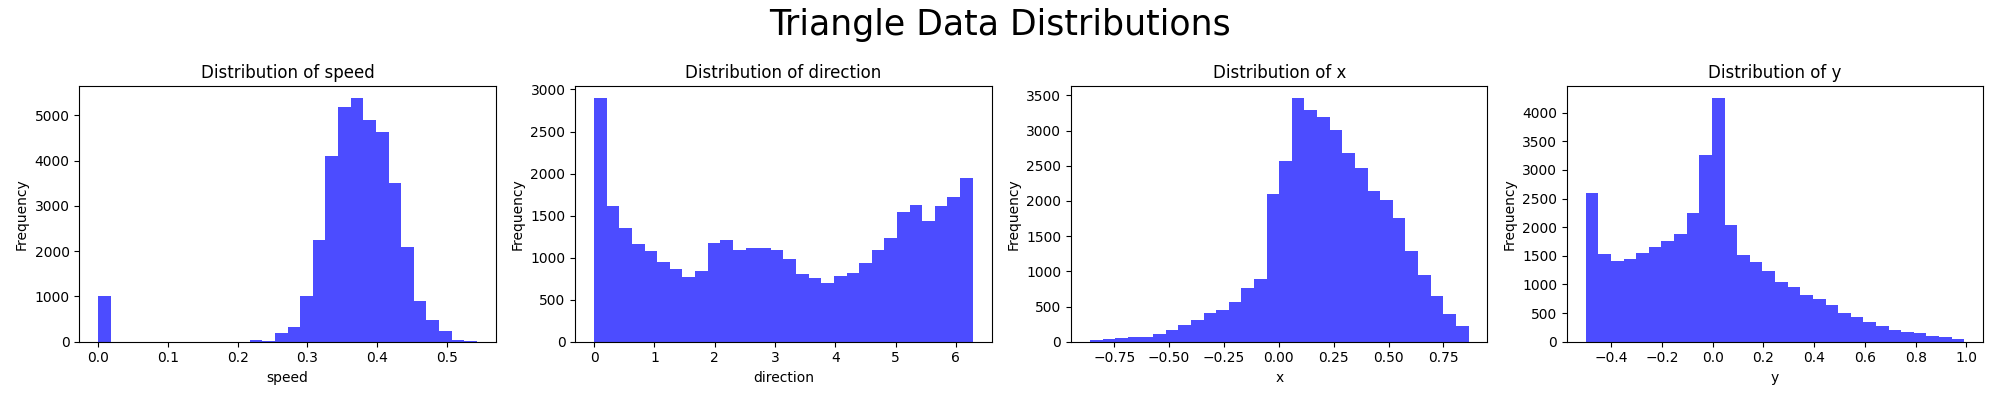
\includegraphics[width=\textwidth]{figures/triangle_data_distribution.png}
    \caption{Triangle environment data distributions for speed, direction, x and y coordinates.}
    \label{fig:triangle_data_distribution}
\end{figure}

\begin{figure}
    \centering
    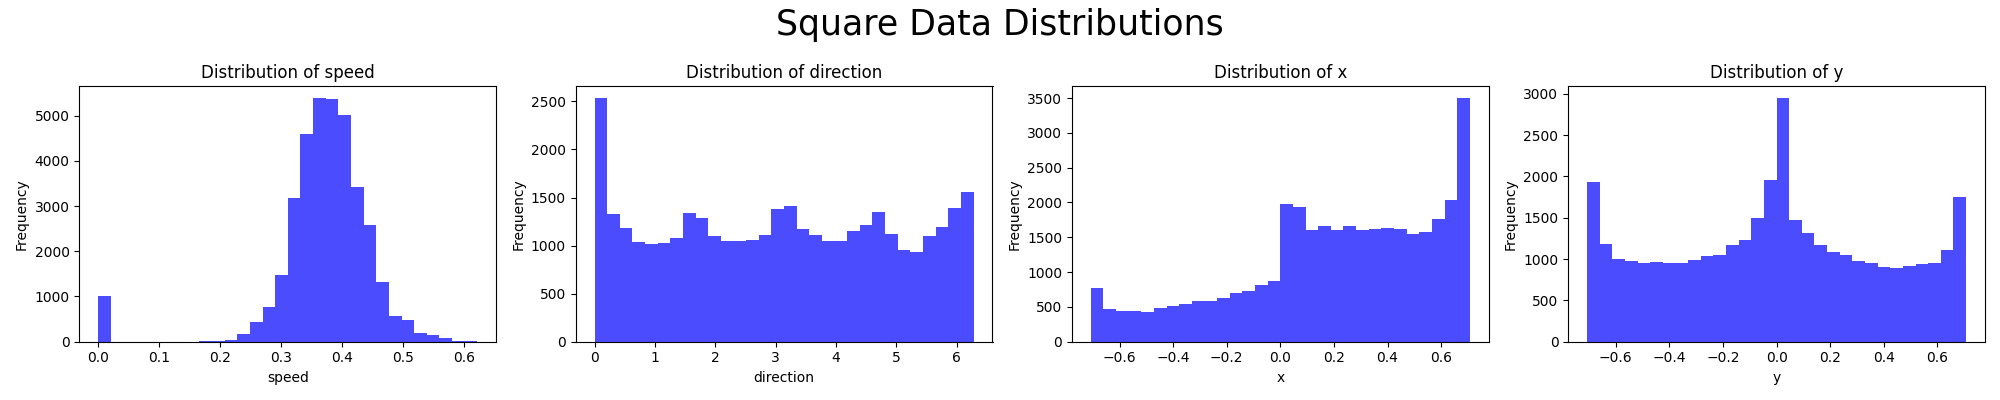
\includegraphics[width=\textwidth]{figures/square_data_distribution.png}
    \caption{Square environment data distributions for speed, direction, x and y coordinates.}
    \label{fig:square_data_distribution}
\end{figure}


\section{RNN model training}
The RNN model architecture and training procedure closely followed the original paper by \cite{chaplot2018active}. The model consisted of a single hidden layer with 100 units and used a tanh activation function. The input to the network was a sequence of speed and direction signals, and the output was the estimated position of the agent in x and y coordinates. The model was trained using backpropagation through time (BPTT) with a mean squared error loss function extended with a regularization term to encourage sparsity in the hidden layer activations.


\begin{align}
\label{eq:rnn_init}
x_0 &= 0, \quad u_0 = \tanh(x_0) = 0, \\[0.5em]
\label{eq:rnn_update}
x_t &= x_{t-1}
  + \frac{\Delta t}{\tau}
    \left(
      -x_{t-1}
      + W_{\mathrm{rec}} u_{t-1}
      + W_{\mathrm{in}} I_t
      + b
      + \xi_t
    \right),
  \quad \xi_t \sim \mathcal{N}(0, \sigma^2 I), \\[0.8em]
\label{eq:rnn_activations}
u_t &= \tanh(x_t), \\[0.5em]
\label{eq:rnn_out}
y_t &= W_{\mathrm{out}} u_t
\end{align}

Equation \ref{eq:rnn_init} shows the initialization of the RNN's hidden state, where $x_0$ is the initial hidden state vector, and $u_0$ is the initial activation vector obtained by applying the tanh activation function to $x_0$, ensuring that the initial prediction aligns with the starting position of the agent at the origin.

Equation \ref{eq:rnn_update} describes the update of the hidden state at each time step $t$. The hidden state $x_t$ is updated based on the previous hidden state $x_{t-1}$, the recurrent weights $W_{\mathrm{rec}}$, the input weights $W_{\mathrm{in}}$, the input vector $I_t$ (which includes speed and direction), a bias term $b$, and a noise term $\xi_t$ sampled from a Gaussian distribution with mean 0 and variance $\sigma^2 I$. The time constant $\tau$ and time step $\Delta t$ control the dynamics of the RNN.

Equation \ref{eq:rnn_activations} defines the activation of the hidden layer at each time step $t>0$. The activation $u_t$ is obtained by applying the tanh activation function to the hidden state $x_t$, introducing non-linearity into the model.

Equation \ref{eq:rnn_out} specifies the output of the RNN at each time step $t$. The output $y_t$ is computed by multiplying the output weights $W_{\mathrm{out}}$ with the activation vector $u_t$. The output $y_t$ represents the estimated position of the agent in x and y coordinates.



\subsection{Loss and regularization}
Authors repeatedly pointed out the importance of regularization for the emergence of grid-like representations in the hidden layer of the RNN. Hence, the loss function used for training the model consisted of three componenets: task loss, L2 regularization loss on the input and output weights, and a firing rate regularization loss on the hidden layer activations. The total loss function is defined in Equation \ref{eq:loss}.
\[
\begin{aligned}
\mathcal{L}_{\text{total}} 
&= \mathcal{L}_{\text{task}} 
   + \lambda_{\text{L2}} \, \mathcal{L}_{\text{L2}} 
   + \lambda_{\text{FR}} \, \mathcal{L}_{\text{FR}} \\[6pt]
\mathcal{L}_{\text{task}} 
&= \frac{1}{M T N_{\text{out}}} 
   \sum_{m=1}^{M} \sum_{t=1}^{T} \sum_{k=1}^{N_{\text{out}}}
   \left( Y_{\text{pred}}^{(m,t,k)} - Y_{\text{target}}^{(m,t,k)} \right)^2 \\[6pt]
\mathcal{L}_{\text{L2}} 
&= \frac{1}{N N_{\text{in}}} \sum_{i=1}^{N} \sum_{j=1}^{N_{\text{in}}} 
   (W_{\text{in},ij})^2
   + \frac{1}{N_{\text{out}} N} \sum_{k=1}^{N_{\text{out}}} \sum_{i=1}^{N}
   (W_{\text{out},ki})^2 \\[6pt]
\mathcal{L}_{\text{FR}} 
&= \frac{1}{M T N} \sum_{m=1}^{M} \sum_{t=1}^{T} \sum_{i=1}^{N} 
   U_{mti}^2
\label{eq:loss}
\end{aligned}
\]

\section{Results}
The RNN models were trained separately on the triangle and square environment datasets. The training process involved optimizing the total loss function defined in Equation \ref{eq:loss} using backpropagation through time (BPTT). The models were trained for a total of 1500 epochs, with the training loss being monitored throughout the process. The training loss curves for both models are shown in Figure \ref{fig:loss_curves}. 

\begin{figure}
    \centering
    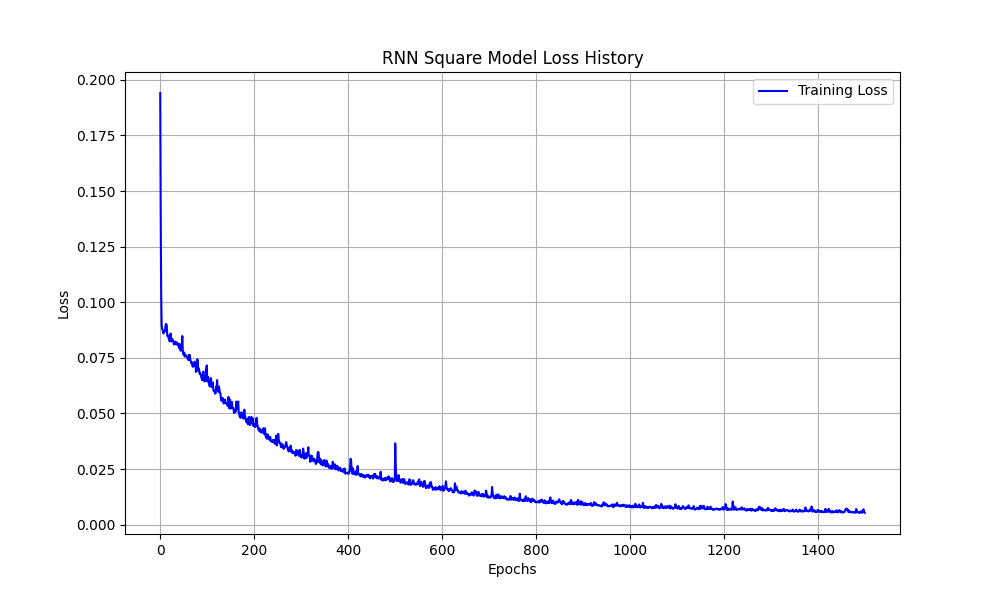
\includegraphics[width=\textwidth]{figures/rnn_square_model_loss_history.png}
    \caption{Training loss curves for RNN models trained on a square environment.}
    \label{fig:loss_curves}
\end{figure}



\section{Discussion}



\bibliography{references}
\bibliographystyle{apacite}
\end{document}